\documentclass[11pt,a4paper]{article}
\usepackage[a4paper,margin=20mm,headheight=14pt]{geometry}
\usepackage[T1]{fontenc}
\usepackage[utf8]{inputenc}
\usepackage{lmodern,amsmath,amssymb,graphicx,booktabs,tabularx,longtable,array}
\usepackage{microtype,caption,float,hyperref,fancyhdr}
\hypersetup{hidelinks}
\captionsetup{font=small,labelfont=bf}
\setlength{\parskip}{4pt}\setlength{\parindent}{0pt}
\setlength{\emergencystretch}{1.5em}
\graphicspath{{figures/}}
\makeatletter\def\input@path{{tables/}}\makeatother
\pagestyle{fancy}\fancyhf{}\fancyhead[L]{\small PyEXPINT | supplementary material}\fancyhead[R]{\small Supplementary material}\fancyfoot[C]{\thepage}
\renewcommand{\headrulewidth}{.3pt}
\renewcommand{\tabularxcolumn}[1]{>{\raggedright\arraybackslash}p{#1}}

\renewcommand{\thetable}{S\arabic{table}}
\renewcommand{\thefigure}{S\arabic{figure}}
\begin{document}
\title{PyEXPINT: Supplementary Material}
\author{}\date{}
\maketitle

\paragraph{Scope.} This supplement contains the development records and the complete
tables behind the main text. The numerical panels are produced by
\path{figure_sources/make_figures.py}.  The script
\path{tables/make_tables.py} regenerates the catalogue, Lawson, startup and
development step-doubling tables; other tables are supplied as LaTeX with
the associated records where available.  Supplementary Table~S6 is generated
separately from the unchanged cross-check summary by
\path{tables/make_crosscheck_table.py}.  These are postprocessing operations,
not new integrator executions. The development records are retained because they document the
design decisions; their protocols differ from the canonical ones and they are not
substitutes for the experiments of the main text.

\section*{Development crossovers}
These records explain why interchangeable realizations and machine-local
measurement are useful; they are not substituted for the canonical campaigns. The
three panels have different measurement protocols, and the selector is excluded
from these time ratios so that a hidden difference between a selected backend and
an explicit backend is not presented as selector overhead. A ratio of medians is
not a median of paired ratios; the canonical campaigns of the main text use the
latter.

\begin{figure}[p]\centering
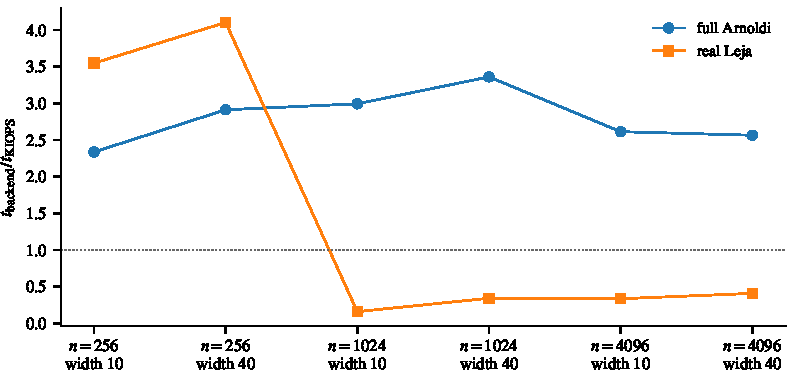
\includegraphics[width=.86\linewidth]{figS01a_crossover_1d.pdf}\\[3pt]
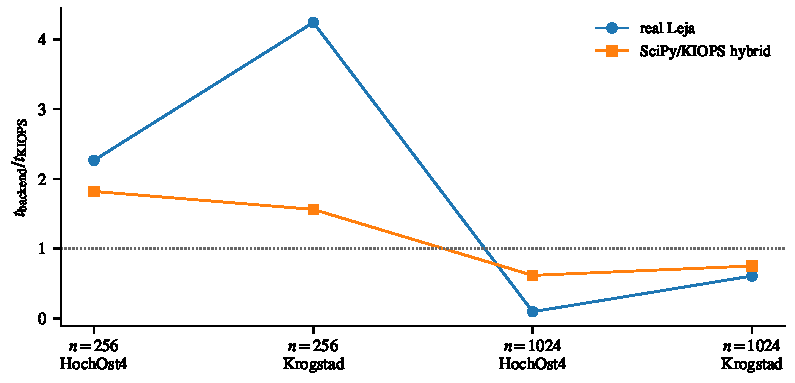
\includegraphics[width=.86\linewidth]{figS01b_hybrid_development.pdf}\\[3pt]
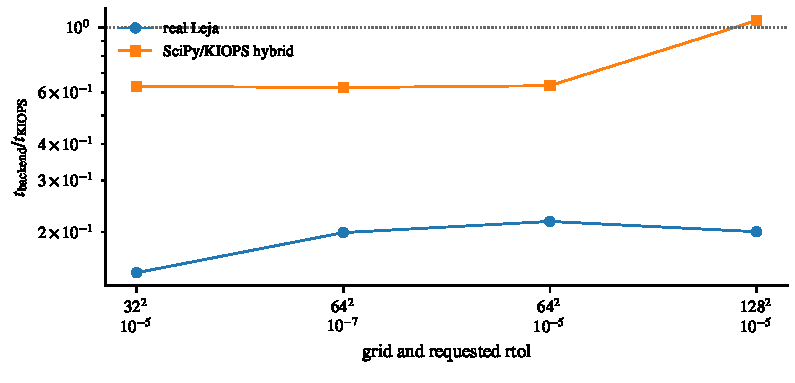
\includegraphics[width=.86\linewidth]{figS01c_prerelease_2d.pdf}
\caption{Development timing records not used in the canonical campaigns. Top: six
one-dimensional cases with the Krogstad scheme and scaled spectral widths 10 and
40 (\texttt{crossover\_phase5.json}). Middle: the hybrid-backend comparison
(\texttt{hybrid\_phase6.json}). Bottom: the pre-release two-dimensional experiment
with three measured repetitions, recorded with Python 3.13.5, NumPy 2.3.5 and
SciPy 1.17.0 rather than the production stack
(\texttt{prerelease\_2d\_selected\_fields.json}). In every panel the denominator is
the KIOPS-type time of the same case. No crossover boundary is inferred between
points, and these ratios are neither paired estimates nor backend rankings.}
\end{figure}\clearpage

\section*{Fixed-step method campaign}
Figure~\ref{fig:supp-replay} shows the complete fixed-step campaign of the main
text: 511 interior points, fixed KIOPS-type action tolerance $10^{-13}$, exact
history, the common numerical window $[0.5,1]$, 27 methods and four step sizes,
108 rows in total (\texttt{method\_wp\_replay2341311\_all.csv}). Enlarged open
markers identify points at or below the precision cutoff $5\times10^{-12}$, tied
to the action tolerance, and are excluded from the non-dominated curves.

\begin{figure}[p]\centering
\begin{minipage}[c]{0.74\linewidth}\centering
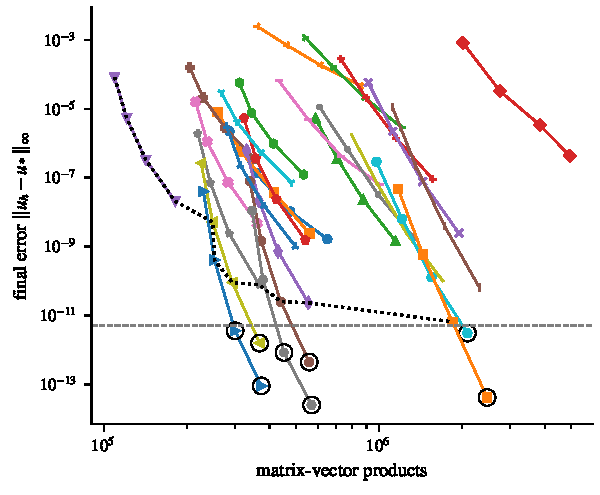
\includegraphics[width=\linewidth]{figS02c_replay_all_matvecs.pdf}\\[6pt]
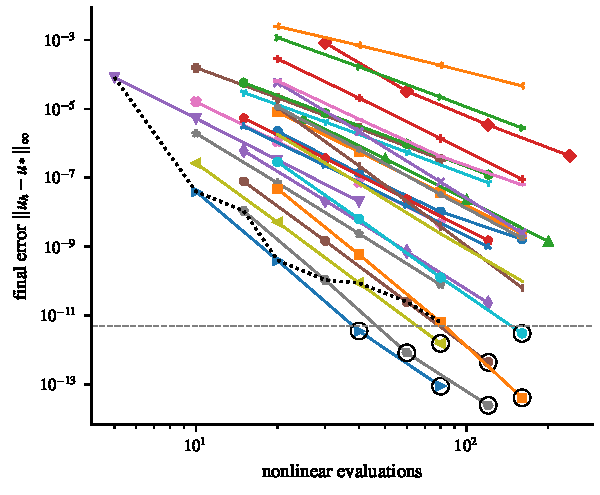
\includegraphics[width=\linewidth]{figS02d_replay_all_nonlinear_evals.pdf}
\end{minipage}\hfill
\begin{minipage}[c]{0.24\linewidth}\centering
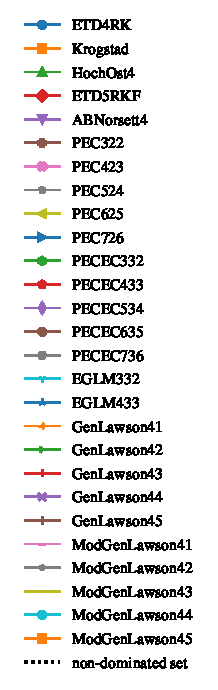
\includegraphics[width=\linewidth]{figS02e_replay_legend.pdf}
\end{minipage}
\caption{The fixed-step campaign with all 27 methods and four step sizes. Top:
final error versus matrix-vector products. Bottom: final error versus nonlinear
evaluations. The legend on the right applies to both panels; the eight methods
selected in the main text are a subset of these curves.}\label{fig:supp-replay}
\end{figure}\clearpage

\section*{Temporal and action tolerances}
Figure~\ref{fig:supp-tol} retains the tolerance-coupling sweep that motivated the
separation of temporal and action tolerances in the adaptive solvers. It was
produced with the generic step-doubling controller (\texttt{solve\_adaptive}) and
the Krogstad scheme on a periodic problem with 128 unknowns and $T=1$
(\texttt{action\_tolerance.json}); the action tolerance is a fraction $f$ of the
requested relative tolerance, and the achieved error and the recorded products are
shown against $f$. ETD34 uses the same coupling policy, written explicitly here to avoid
a fragile equation-number reference to the separate article:
\[
 \tau_{\mathrm{act}}=\min(\tau_{\max},
 \max(\tau_{\min},f\,\mathrm{rtol})).
\]

\begin{figure}[htbp]\centering
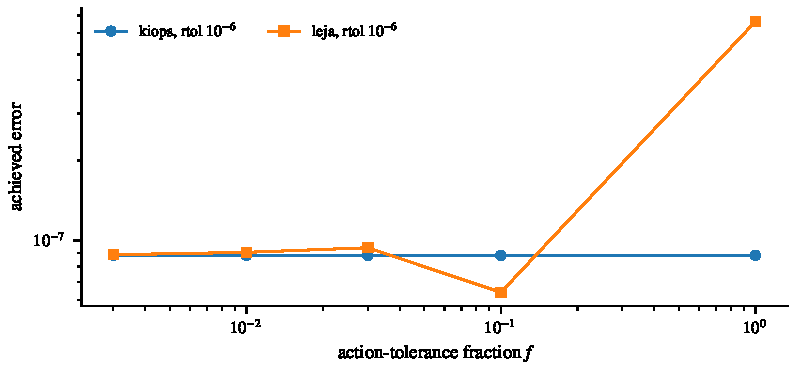
\includegraphics[width=.84\linewidth]{figS03a_action_error_inf.pdf}\\[6pt]
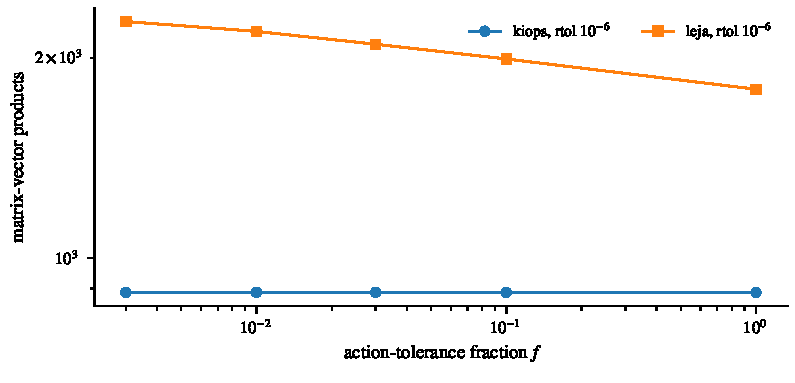
\includegraphics[width=.84\linewidth]{figS03b_action_matvecs.pdf}
\caption{Tolerance-coupling sweep with the step-doubling controller. Top: achieved
error. Bottom: recorded matrix-vector products. Both versus the action fraction
$f$ for the KIOPS-type and real-Leja realizations.}\label{fig:supp-tol}
\end{figure}\clearpage

\section*{Catalogue coverage}
Table~\ref{tab:catalogue47} is the complete record of the 47 entries, with the
provenance of their canonical coefficients, their order metadata and the outcome
of the cross-check against the original EXPINT file of the same name.
The complementary machine-readable index
\path{reproducibility/coverage/catalogue_test_map.csv} lists the source
definitions and concrete test identifiers supporting each entry, with the
limitations described in its README.
\input{tableS01_catalogue.tex}
\clearpage

\section*{Generic convergence of the generalized Lawson families}
Table~\ref{tab:lawson} reports the classical convergence of the generalized and
modified generalized Lawson entries, with Krogstad, HochOst4 and ETD5RKF as
controls, on a generic six-dimensional system with exact history. The slopes of
GenLawson44 and GenLawson45 decrease towards their recorded orders 4 and 5 here,
whereas on the parabolic problem of the main text they rise towards 5 and 6; the
recorded orders are kept and the parabolic behaviour is reported as
problem-dependent.
\input{tableS02_lawson.tex}
\clearpage

\section*{Canonical timing summaries}
Table~\ref{tab:picasso72} lists the 72 configuration summaries of the three
canonical campaigns, one row per replica, grid, tolerance and backend, with the
achieved error and the work counters beside the time
(\texttt{canonical\_summary\_72.csv}). The paired ratios of the main text are
computed within blocks from the raw repetitions
(\texttt{canonical\_paired\_ratios.csv}), not from these medians.
\begingroup\small
\input{tableS03_picasso.tex}\endgroup
\clearpage

\section*{Adaptive and cost-aware diagnostics}
Table~\ref{tab:adaptive-extra} reports the stiff adaptive comparisons of ETD34
with step doubling on the local and nonlocal manufactured problems, and the
cost-aware stress test (\texttt{tableS04a\_stiff.csv}, \texttt{tableS04b\_cost.csv}).
As discussed in the main text, a state-independent additive source
cancels directly from the same-time nonlinear difference in the ETD34
estimator.  When $N(t,y)=g(t)+F(y)$, the source can still influence that
difference through the stage states and $F$.  These records do not isolate
that indirect effect or establish a causal decomposition of the error.
\input{tableS04_adaptivity.tex}

\section*{Step-doubling records of a development experiment}
Table~\ref{tab:phase6} lists the records of an earlier development experiment
with the generic step-doubling controller, two requested tolerances per method
and backend (\texttt{phase6\_work\_precision\_selected\_fields.json}). They are
shown as a table because two points per series do not support a curve.
\input{tableS05_adaptive_records.tex}

\clearpage
\section*{Archived cross-check}
The unchanged report at
\path{reproducibility/expint_crosscheck/crosscheck_report.txt} supplies
Table~S6.  The same directory additionally contains 102 numerical-output
rows, coefficient values, refinement output, the correction diffs, selected
original-source hashes and copies of both comparison drivers.  The drivers'
original runnable location is in the private software companion, where the
Python comparison resolves its source imports.  Original EXPINT MATLAB
files are not redistributed.  The coefficient indices in the drivers are
one-based.  Equality at two configurations is not an order theorem.
\input{tableS06_crosscheck.tex}
\clearpage

\section*{Source boundary}
Selected plotting records are under \path{reproducibility/t8_data}; the
original Allen--Cahn record in that directory is byte-identical to the
workstation JSON in the private companion.  Its old provisional
transcription is retained only in the revision history and is not plotted.
The private archive \path{pyexpint_review_package_20261011.zip} contains the
source snapshot, wheel/sdist, tests, examples, drivers and detailed logs.
The associated evidence index and coverage map identify those paths and
separate original experiment outputs, logged candidate comparisons and
manuscript postprocessing.  No new integration, test-suite run or public
software release is implied by this manuscript revision.
\end{document}
